\documentclass[a4paper,12pt]{article}

\usepackage[top = 2cm, bottom = 2cm, left = 2cm, right = 2cm]{geometry} 

\usepackage[T1]{fontenc}
\usepackage[utf8]{inputenc}
\usepackage[spanish]{babel}
\usepackage{multirow}
\usepackage{booktabs} 
\usepackage{graphicx} 
\usepackage{setspace}
\setlength{\parindent}{0in}
\usepackage{float}
\usepackage{fancyhdr}
\usepackage{enumitem}
\usepackage{tikz-timing}
\usepackage{amsmath,amssymb,amsfonts}
\usepackage[thinlines]{easytable}
\usepackage{array}
\usepackage{listings}
\usepackage{hyperref} % Support for hyperlinks
\usepackage{xcolor}
\usepackage{pdflscape}

\definecolor{LightGray}{gray}{0.95}

\definecolor{mGreen}{rgb}{0,0.4,0}

\lstset{
    frame=tblr, % draw a frame at the top and bottom of the code block
    tabsize=4, % tab space width
    showstringspaces=false, % don't mark spaces in strings
    numbers=left, % display line numbers on the left
    commentstyle=\color{mGreen}, % comment color
    keywordstyle=\color{blue}, % keyword color
    stringstyle=\color{red}, % string color
    linenos=true,
    breaklines
}


\tikzset{
timing/z/.style={color=red},
timing/l/.style={color=red},
timing/h/.style={color=red},
timing/slope=0,
timing/name/.append style={yshift=1.5mm}
}

\pagestyle{fancy} 
\lhead{\footnotesize Construcción de Software: Laboratorio 9}

\rhead{\footnotesize 04 de diciembre del 2020}

\cfoot{\footnotesize \thepage} 

\begin{document}

\thispagestyle{empty}

\begin{tabular}{p{15.5cm}} 
\large Universidad Nacional de San Agustín \\ 
\large Facultad de Ingeniería de Producción y Servicios \\
\large Escuela Profesional de Ingeniería de Sistemas \\
{\LARGE \bf Construcción de Software} \\
\vspace{1mm}
Alumno: Mestas Escarcena, Carlos Alberto \\
Grupo: B \\
\hline \\
\end{tabular} 

\begin{center} 
	{\LARGE \bf Laboratorio 9 - UML aplicado}
	\vspace{2mm}
\end{center}  

En desarrollo de los diferentes diagramas se realizó con  \textcolor{blue}{
    \href{https://www.planttext.com/}{PlantText UML Editor}}.
\\
\\
En desarrollo del informe se encuentra en \textcolor{blue}{
    \href{https://github.com/CarlosMestas/CS_CarlosMestas_Laboratorio_9}{GitHub}}.

\section*{Ejercicio 1}

\begin{itemize}
    \item 11. El 16 de noviembre Francisco Sagasti es elegido como presidente del congreso de la República del Perú.
    \item 12. El 17 de noviembre juramenta como presidente constitucional del Perú. La ONU felicita a Francisco Sagasti como presidente del Perú.
    \item 13. El 18 de noviembre distintos congresistas se pronuncian sobre el fallecimiento de los jóvenes en las protestas
\end{itemize}

\section*{Ejercicio 2}

El código utilizado para generar el diagrama fue:

\begin{lstlisting}
@startuml

title UML Aplicado - Diagrama de Casos de Uso 

(Elecciones) as z1
(Derecho a protestar) as z2
(Protección) as z3


actor :Ciudadano: as ciu
actor :Poder Legislativo: as podleg
actor :Poder Judicial: as podjud
actor :Poder Ejecutivo: as podeje
actor :Fuerzas Armadas: as fuearm

(Promulgar leyes) as a1
(Ejercer el\nderecho de\namnistía) as a2
(Autorizar viajes\nal Presidente\nfuera del país) as a3

podleg --> a1
podleg --> a2
podleg --> a3

(Cumplir y hacer\ncumplir la\nconstitución) as b1
(Velar por el\norden interno\ny la seguridad\nexterior de la\nRepublica) as b2
(Convocar a elecciones) as b3
(Decretar\nestado de emergencia) as b4
(Disolver\nel congreso) as b5
(Designa ministros) as b6
(Pedido de confianza) as b7

podeje --> b1
podeje --> b2
podeje --> b3
podeje --> b4
podeje --> b5
podeje --> b6

b3 ..> ciu : include
b4 ..> ciu : include

b6 ..> b7 : include

(Juzgar a quienes\ninclumpan las leyes) as c1

podjud --> c1

c1 ..> ciu : include

ciu --> z1 : participa en
ciu --> z2 

z1 ..> podeje : include
z1 ..> podleg : include

fuearm --> z3
z3 ..> ciu : include

@enduml
\end{lstlisting}

\clearpage
\newpage
    
    \begin{landscape}
    

\begin{figure}[p]
        \centering        
        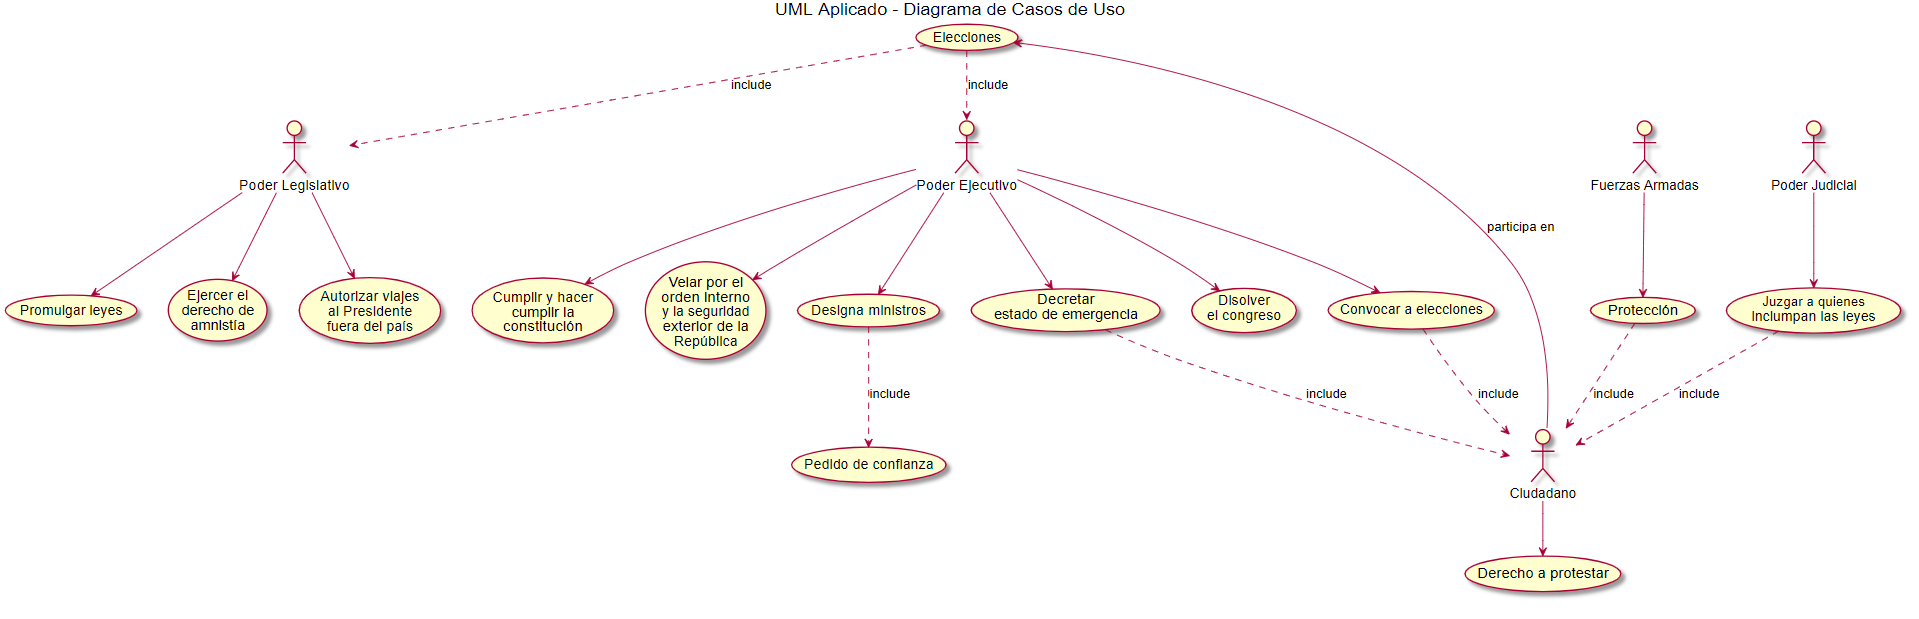
\includegraphics[width=1.5\textwidth]{images/umlA01.PNG}
        \caption{Diagrama de casos de Uso - Ejercicio 2.}  
        {{\footnotesize Realizado en: PlantText UML Editor }}
\end{figure}

    \end{landscape}

\clearpage
\newpage

\section*{Ejercicio 3}

El código utilizado para generar el diagrama fue:

\begin{lstlisting}
@startuml

title "UML Aplicado - Diagrama de secuencia"

actor "Congreso" as a3
actor "Vizcarra" as a1
actor "Abogado" as a2
actor "Diario el Peruano" as a4


activate a3

a3 ->> a3 : 1. Se da el pedido de vacancia

alt Firmas de congresistas > 26

a3 ->> a3 : 2. Se brindan fundamentos


a3 ->> a1 : 3. Se emite una copia


activate a1
deactivate a1

    alt Admision del pedido de vacancia > 52 votos
    
        a3 ->> a3 : 4. Se acuerda el dia y hora para el debate y el pedido de vacancia
    
        a3 ->> a1 : 5. Se le informa
        activate a1
        deactivate a1
      
    end

    a3 ->> a3: 6. Comienza el debate
    
    a3 ->> a1: 7. Se le permite su defensa
    activate a1
    
    alt Cuenta con abogado
    
        a1 ->> a1: 8. Ejerce su defensa
    
    else No cuenta con abogado
    
        a1 ->> a2: 9. Le da pase a su abogado
        deactivate a1
        activate a2

        
        a2 ->> a2: 10. Expone la defensa
        deactivate a2
    end
    
    
    a3 ->> a3 : 11. Comienza la votacion
    
    alt Votos > 87
    
        a3 ->> a3 : 12. Se aprueba la vacancia
        
        a3 ->> a4 : 13. Informa
        activate a4
        
        a4 ->> a4 : 14. Realiza la publicación
        deactivate a4
        
    else 
    
        a3 ->> a3 : 15. Se rechaza la vacancia
        
    end
    
end
\end{lstlisting}

\clearpage
\newpage
    
 %   \begin{landscape}
    

\begin{figure}[p]
        \centering        
        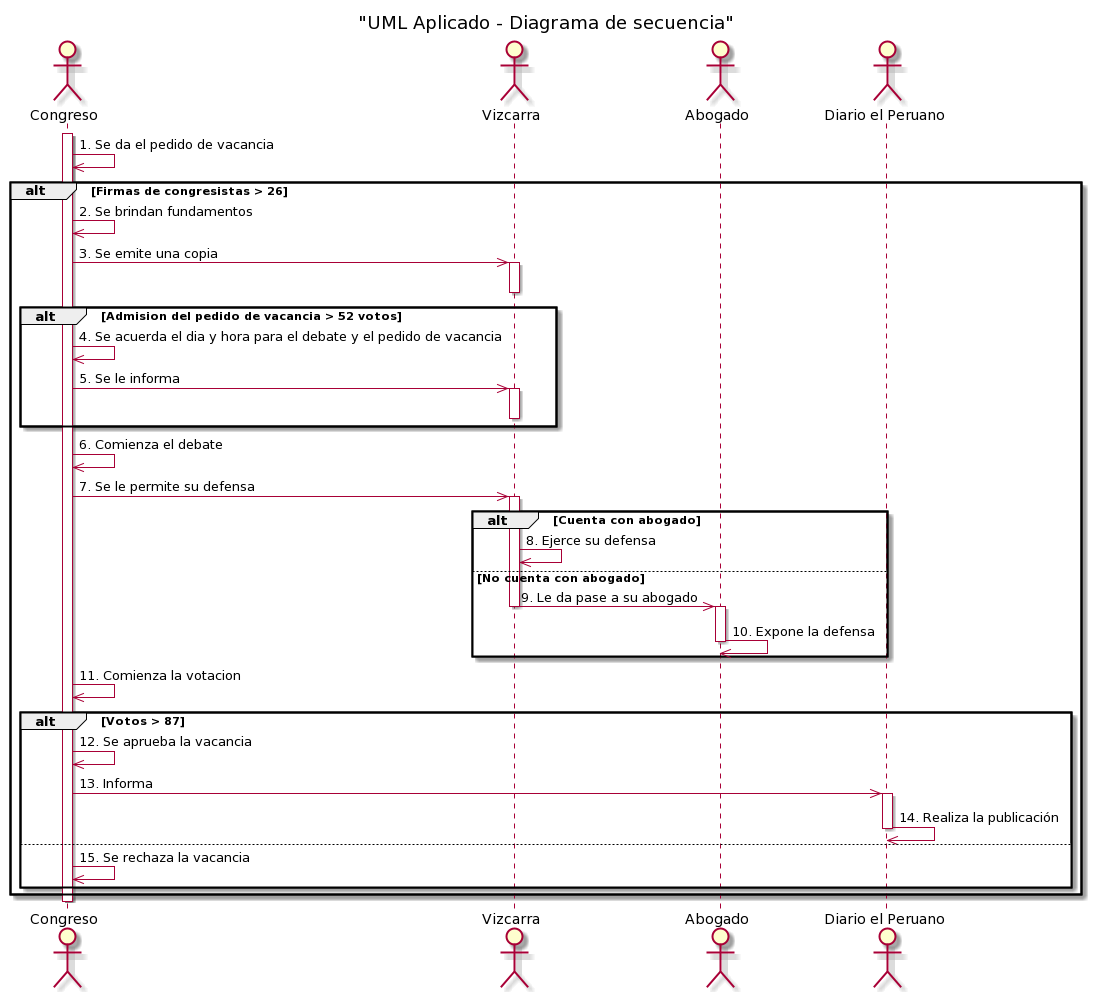
\includegraphics[width=1\textwidth]{images/umlA02.PNG}
        \caption{Diagrama de secuencia - Ejercicio 3.}  
        {{\footnotesize Realizado en: PlantText UML Editor }}
\end{figure}

  %  \end{landscape}
    
\clearpage
\newpage

\section*{Ejercicio 4}

El código utilizado para generar el diagrama fue:

\begin{lstlisting}
@startuml

title "UML Aplicado - Diagrama de secuencia"

actor "Congreso" as a3
actor "Vizcarra" as a1
actor "Abogado" as a2
actor "Diario el Peruano" as a4


activate a3

a3 ->> a3 : 1. Se da el pedido de vacancia

alt Firmas de congresistas > 26

a3 ->> a3 : 2. Se brindan fundamentos


a3 ->> a1 : 3. Se emite una copia


activate a1
deactivate a1

    alt Admision del pedido de vacancia > 52 votos
    
        a3 ->> a3 : 4. Se acuerda el dia y hora para el debate y el pedido de vacancia
    
        a3 ->> a1 : 5. Se le informa
        activate a1
        deactivate a1
      
    end

    a3 ->> a3: 6. Comienza el debate
    
    a3 ->> a1: 7. Se le permite su defensa
    activate a1
    
    alt Cuenta con abogado
    
        a1 ->> a1: 8. Ejerce su defensa
    
    else No cuenta con abogado
    
        a1 ->> a2: 9. Le da pase a su abogado
        deactivate a1
        activate a2

        
        a2 ->> a2: 10. Expone la defensa
        deactivate a2
    end
    
    
    a3 ->> a3 : 11. Comienza la votacion
    
    alt Votos > 87
    
        a3 ->> a3 : 12. Se aprueba la vacancia
        
        a3 ->> a4 : 13. Informa
        activate a4
        
        a4 ->> a4 : 14. Realiza la publicación
        deactivate a4
        
    else 
    
        a3 ->> a3 : 15. Se rechaza la vacancia
        
    end
    
end
\end{lstlisting}


 %   \begin{landscape}
    
\clearpage
\newpage

\begin{figure}[ht]
        \centering        
        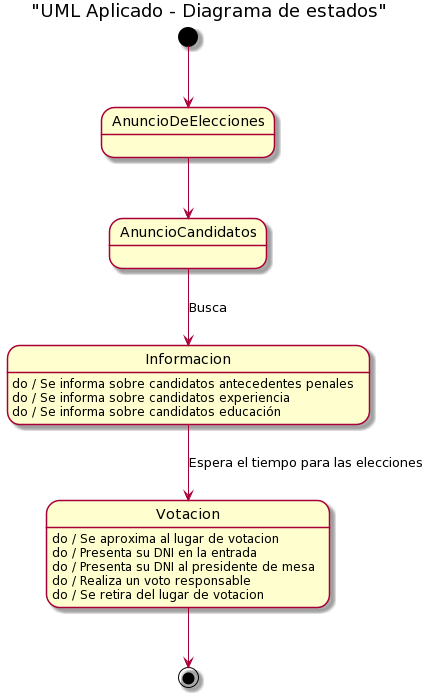
\includegraphics[width=0.5\textwidth]{images/umlA03.PNG}
        \caption{Diagrama de estados - Ejercicio 4.}  
        {{\footnotesize Realizado en: PlantText UML Editor }}
\end{figure}


\begin{thebibliography}{00}

\bibitem{b0} Ec, R. (2019, October 1). \textit{¿Cuál es el procedimiento para la vacancia presidencial?} El Comercio Perú. https://elcomercio.pe/politica/congreso/cual-es-el-procedimiento-para-la-vacancia-presidencial-noticia/

\end{thebibliography}


\clearpage
\newpage



\clearpage
\newpage





    
\end{document}
